\documentclass[10pt, border=3mm]{standalone}
\usepackage{pstricks-add}
\usepackage{tikz}
\usetikzlibrary{positioning, calc, graphs}

\begin{document}

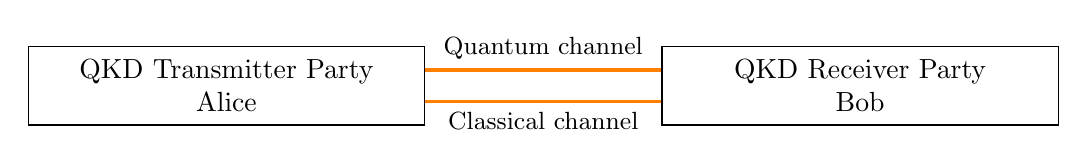
\begin{tikzpicture}[block/.style={rectangle,draw,minimum height=1cm,text width=4.8cm,align=center},node distance = 30mm ]
\node (b1) [block] {QKD Receiver Party\\Bob} ;
\node (b2) [block,left=of b1] {QKD Transmitter Party\\ Alice};
  \begin{scope}
   % \draw[double distance=20pt] (b1) -- node [sloped, above] {\small{Quantum channel }} (b2);
    \draw [-, orange, very thick] ($(b1.west)+(0,-0.2)$) -- node [below, black] {\small{Classical channel }} ($(b2.east)+(0,-0.2)$);
    \draw [-, orange, very thick] ($(b1.west)+(0,0.2)$) -- node [above, black] {\small{Quantum channel }} ($(b2.east)+(0,.2)$);
  \end{scope}
\end{tikzpicture}
\end{document}